\documentclass[tikz,border=5pt]{standalone}
\usepackage{luatexja}
\usepackage[hiragino-pron]{luatexja-preset}
\usepackage{amsmath,amssymb}
\usetikzlibrary{arrows.meta,patterns}

\begin{document}
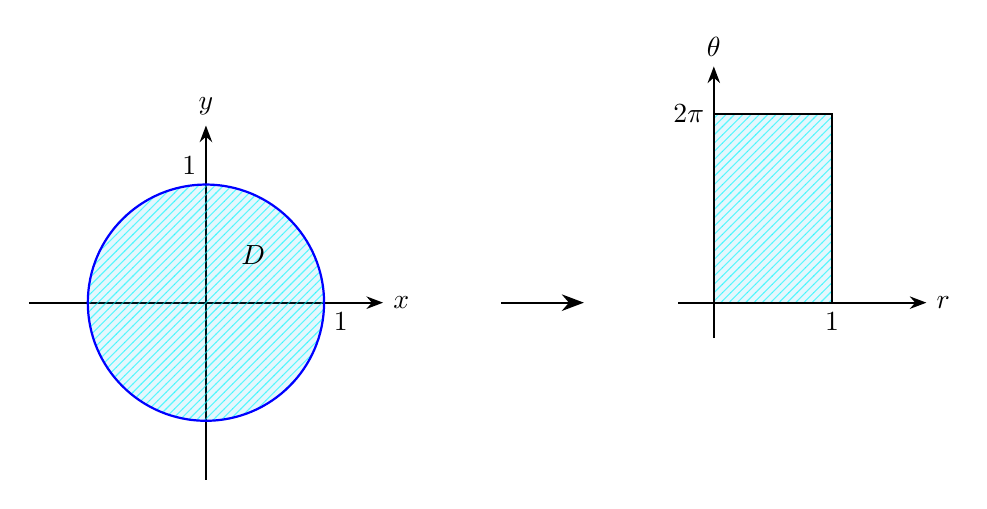
\begin{tikzpicture}[scale=1.5]

% D region (xy-plane)
\begin{scope}
  % Axes
  \draw[-{Stealth[length=6pt]}, thick] (-1.5,0) -- (1.5,0) node[right] {$x$};
  \draw[-{Stealth[length=6pt]}, thick] (0,-1.5) -- (0,1.5) node[above] {$y$};

  % Unit circle fill
  \fill[pattern=north east lines, pattern color=cyan, opacity=0.6]
    (0,0) circle (1);
  \fill[cyan, opacity=0.1]
    (0,0) circle (1);

  % Unit circle border
  \draw[thick, blue] (0,0) circle (1);

  % Labels
  \node[below right] at (1,0) {$1$};
  \node[above left] at (0,1) {$1$};
  \node at (0.4,0.4) {$D$};
\end{scope}

% Arrow
\draw[-{Stealth[length=8pt]}, thick] (2.5,0) -- (3.2,0);

% E region (r-theta plane)
\begin{scope}[shift={(4.3,0)}]
  % Axes
  \draw[-{Stealth[length=6pt]}, thick] (-0.3,0) -- (1.8,0) node[right] {$r$};
  \draw[-{Stealth[length=6pt]}, thick] (0,-0.3) -- (0,2.0) node[above] {$\theta$};

  % Rectangle E
  \fill[pattern=north east lines, pattern color=cyan, opacity=0.6]
    (0,0) rectangle (1,1.6);
  \fill[cyan, opacity=0.1]
    (0,0) rectangle (1,1.6);
  \draw[thick] (0,0) rectangle (1,1.6);

  % Labels
  \node[below] at (1,0) {$1$};
  \node[left] at (0,1.6) {$2\pi$};
\end{scope}

\end{tikzpicture}
\end{document}
